\hypertarget{baalbeck-au-revoir-liban}{%
\section{Baalbeck \& au revoir, Liban
!}\label{baalbeck-au-revoir-liban}}

\emph{Vendredi 25 mai 2018}

Le point d'orgue de nos derniers jours au Liban a été la visite des
ruines de Baalbeck. Ces ruines, dont l'origine remonte aux romains, sont
extrêmement impressionnantes. Dans les presques vingt siècles qui ont
suivis leur construction, elles ont été réutilisées par les différents
peuples qui ont habité cette région. Jusqu'à aujourd'hui, puisque le
site est utilisé pour accueillir le festival international de musique de
Baalbeck.

\begin{figure}
\centering
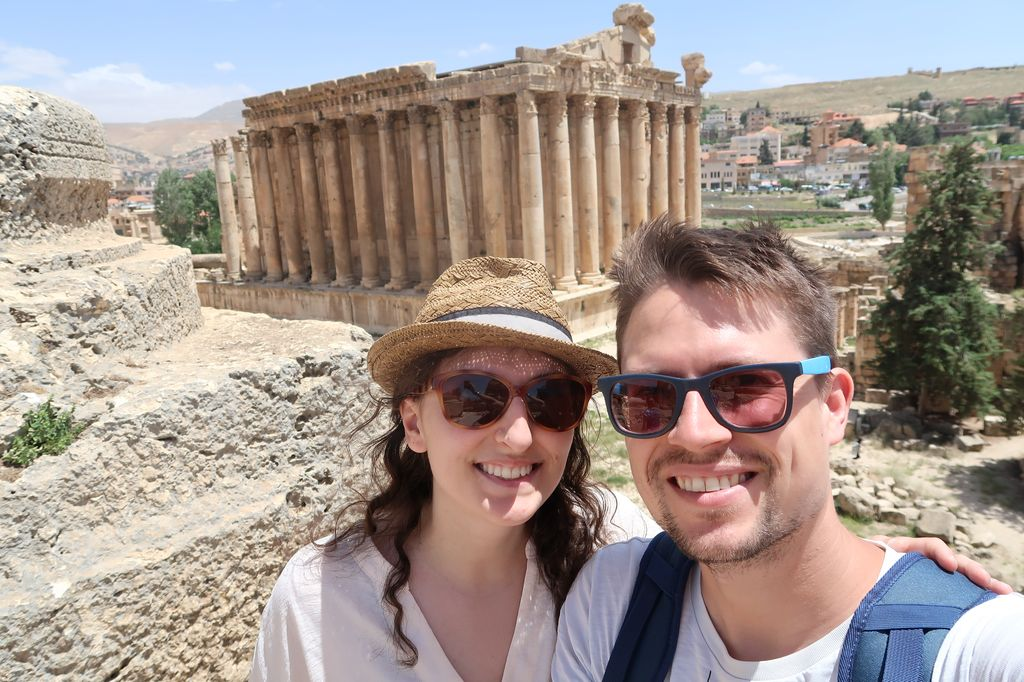
\includegraphics{images/20180525_baalbeck.JPG}
\caption{La vue sur le temple de Bacchus.}
\end{figure}

Ce qui frappe lorsqu'on visite le site, c'est l'ampleur des
installations romaines, construites sur plusieurs siècles. On distingue
l'édifice principal ("temple de Jupiter") dont les six colonnes
d'environ 20 mètres sont emblématiques et le temple dit de Bacchus, le
mieux conservé. Les pierres sont si grandes qu'on se pose immédiatement
la question des techniques de construction utilisées. Cela dit, il
semblerait qu'il n'y ait pas besoin d'invoquer de forces
extra-terrestres à cet endroit, mais bien la présence de nombreux bras,
boeufs et de systèmes de poulie comme expliqué dans
\href{http://www.persee.fr/doc/syria_0039-7946_1977_num_54_1_6623}{cet
article de 1977}.

Les derniers jours au Liban, nous les avons passés à Saghbine, à l'abri
du soleil qui tape de plus en plus fort et à explorer quelques endroits
alentours : vergers, sources et terres forestières de ce pays qui à la
belle saison regorge de fruits.

Au revoir, Liban ! Ou plutôt : à bientôt. Nous reviendrons :)

\emph{Florian et Elida}

\hypertarget{commentaires}{%
\subsection{Commentaires}\label{commentaires}}

\begin{itemize}
\item
  Pierre Guérold, \emph{2018-06-07 20h57}

  Et voilà que je me retrouve à lire un article sur le levage des
  pierres dans l'antiquité....\\
  C'est juste wahou votre voyage.\\
  Merci :)\\
  Pierre
\item
  Florian LB, \emph{2018-06-08 18h11}

  Trop cool ! Je me demandais qui allait être assez courageux pour
  cliquer sur le lien. J'ai trouvé ce sujet très intéressant, mais j'ai
  pas tout compris. Alors j'espère qu'on pourra en reparler quand on
  sera rentré ! A bientôt !
\end{itemize}
